\documentclass[12pt,a4paper,titlepage]{article}
\usepackage[utf8]{inputenc}
\usepackage[czech]{babel}
\usepackage[T1]{fontenc}
\usepackage{amsmath}
\usepackage{amsfonts}
\usepackage{amssymb}
\usepackage{graphicx}
\usepackage{indentfirst}
\usepackage[T1]{fontenc}
\usepackage{tocloft}
\usepackage{secdot}
\usepackage{courier}
\usepackage{fancyhdr}
\usepackage{enumitem}
\usepackage{program}
\usepackage{booktabs}

\begin{document}

% Úvodní strana

\includegraphics[width = 4cm]{LOGO.png} 
\\[8\baselineskip]
\begin{center}

\LARGE\textbf{Semestrální práce z předmětu KIV/MKZ}\linebreak\linebreak
\Large\textbf{Evropa 2 - přehrávání mp3 záznamů z vysílání}\\[11\baselineskip]
\end{center}

\begin{center}
\begin{tabular}{rll}
Vypracoval: & Roman Zeleník \\ 
Studijní číslo: & A12B0212P \\ 
Orion login: & zelenikr \\ 
Datum: & \multicolumn{2}{l}{30.6.2015} \\ 
\end{tabular} 
\end{center}
\thispagestyle{empty}
\pagebreak 

% Obsah
\renewcommand{\cftsecleader}{\cftdotfill{\cftdotsep}}
\tableofcontents
\thispagestyle{empty}
\pagebreak
\setcounter{page}{1}
%Zadání - co práce řeší
\section{Zadání}
	\paragraph{}
	Vytvořte mobilní aplikaci, která poběží na platformě Android. Aplikace umožní uživateli procházet a přehrávat uložené záznamy vysílání rádia Evropa 2.

%Programátorská dokumentace - použité třídy, nejdůležitější metody, algoritmy
\section{Programátorská dokumentace}
	\subsection{Použité třídy}
	\paragraph{MainActivity}
	- Hlavní třída aplikace a jediná \texttt{Activity} třída. 
	
	\paragraph{AudioController}
	- Obsahuje \texttt{View} všech ovládacích prvků (play, next, previous, seekbar) a informačních prvků (aktuální čas, celkový čas, název, obrázek).
	
	\paragraph{DownloaderFactory}
	- Tovární třída pro vytváření speciálních \texttt{AsyncTask} objektů, které stahují data ze serveru rádia Evropa 2 (seznam kategorií, záznamů, mp3 soubory, obrázky, atd.).
	
	\paragraph{PrepareStream}
	- \texttt{AsyncTask}, který volá nad objektem třídy \texttt{MediaPlayer} metody \texttt{setDataSource()} a \texttt{prepare()}. Tyto metody nastaví a připraví datový proud, pro přehrání záznamu. Pomocí posluchače \texttt{OnPreparedListener} upozorní, že je zdroj připraven ke čtení.
	
	\paragraph{CategoriesAdapter}
	- Adapter pro \texttt{ExpandableListView} a potomek \\ třídy \texttt{BaseExpandableListAdapter}. Spravuje seznam aktuálních i archivních kategorií.

	\paragraph{RecordsAdapter}
	- Adapter pro \texttt{RecyclerView} a potomek třídy \\ \texttt{RecyclerView.Adapter}. Spravuje seznam aktuálně zobrazených záznamů.

	\paragraph{EndlessScrollListener}
	- Potomek rozhraní \\ \texttt{RecyclerView.OnScrollListener} a slouží k automatickému stahování záznamů, pokud se uživatel rolováním v seznamu dostane ke konci seznamu.
	
	\paragraph{Category}
	- Představuje konkrétní kategorii z archivu. Mimo jiné obsahuje množinu všech načtených záznamů, které patří do této kategorie.
	
	\paragraph{Record}
	- Představuje konkrétní záznam v kategorii. Mimo jiné obsahuje url adresu mp3 souboru s nahrávkou.
	
	\paragraph{HttpRequests}
	- Statická třída pro posílání \texttt{http} požadavků na server.	
	
	\paragraph{Extractor}
	- Statická třída, která obsahuje metody pro vyhledávání určitých elementů v html souboru.
	
	\paragraph{HtmlParser}
	- Vytvoří seznam kategorií či záznamů z daného html kódu.

	\paragraph{Parser}
	- Abstraktní třída s pomocnými \uv{parsovacími} metodami.

	\paragraph{CategoryParser}
	- Potomek třídy \texttt{Parser}. Slouží k vytvoření kategorie z html kódu.

	\paragraph{RecordParser}
	- Potomek třídy \texttt{Parser}. Slouží k vytvoření záznamu z html kódu.

	\subsection{Externí knihovny}{
	\paragraph{}
	Použil jsem knihovnu \texttt{jsoup} pro práci s html dokumenty. 
	
\pagebreak
%Uživatelská dokumentace - ovládání aplikace, screenshot aplikace,
%	případné poznámky k instalaci aplikace (pokud je nestandardní)
\section{Uživatelská dokumentace}
	\paragraph{}
	Aplikace je určena pro zařízení se systémem Android 4.1 a vyšší.
	
	\begin{center}
		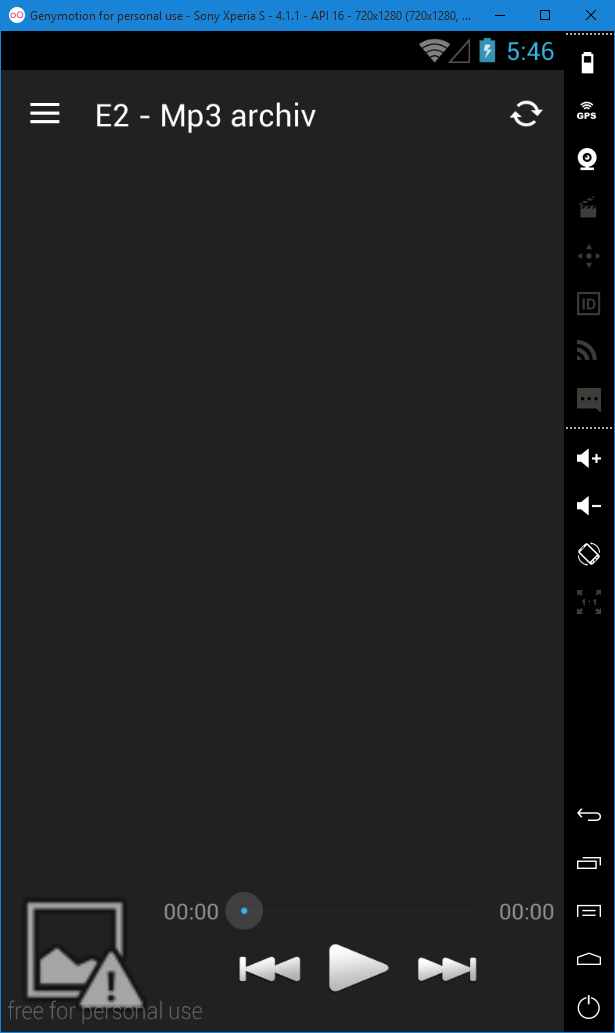
\includegraphics[scale=0.5]{archiv1.png}	
	\end{center}
	\begin{center}
		\footnotesize Obr. 1 - Spuštěná aplikace	
	\end{center}

	V levém menu je seznam všech kategorií. Klepnutím na název kategorie se stáhnou poslední (nejnovější) přidané záznamy. 

	\begin{center}
		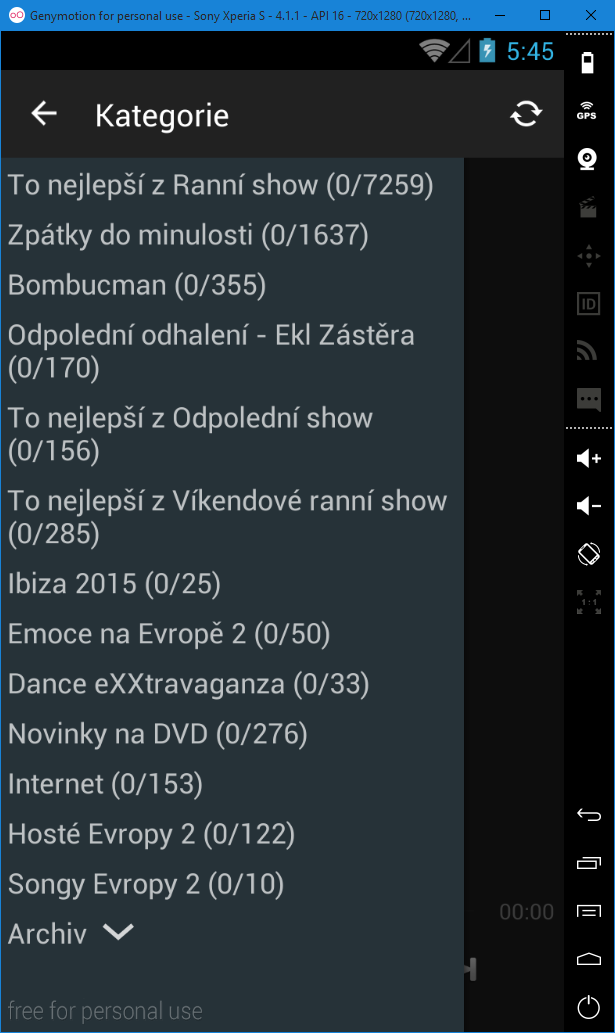
\includegraphics[scale=0.5]{archiv2.png}	
	\end{center}
	\begin{center}
		\footnotesize Obr. 2 - Výběr kategorie	
	\end{center}
	
	Záznamy jsou řazeny abecedně od nejnovějších. Další se stahují automaticky při posouvání seznamu dolu.	
	
	\begin{center}
		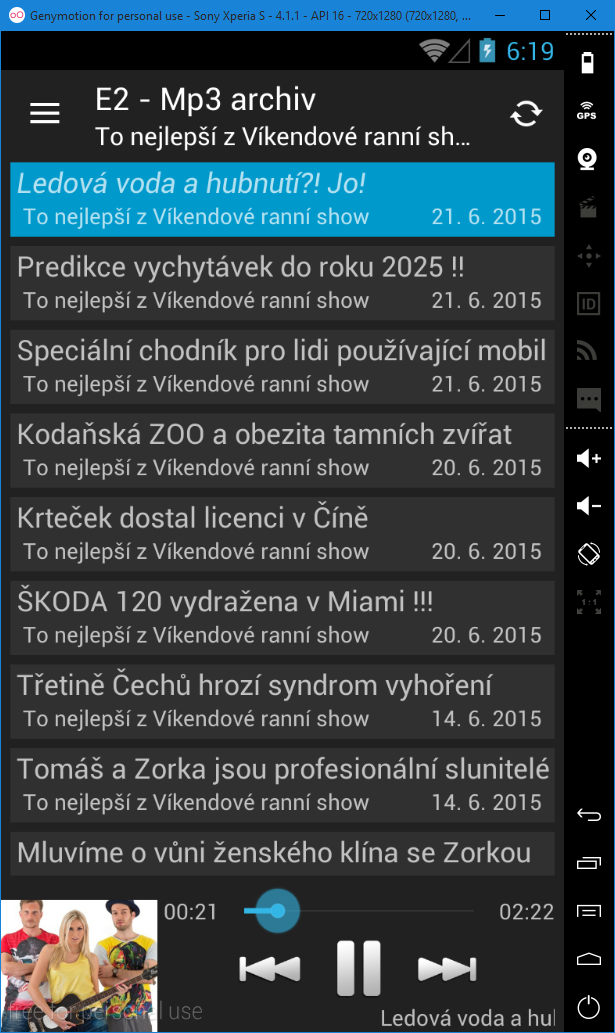
\includegraphics[scale=0.5]{archiv3.png}	
	\end{center}
	\begin{center}
		\footnotesize Obr. 3 - Přehrávání záznamu	
	\end{center}
	
	Po klepnutí na položku v seznamu se mp3 soubor začne načítat ze serveru, a pak se sám spustí. Přehrávaní je možné ovládat tlačítky pod seznamem. Můžete jej pozastavit, přeskočit na další položku v seznamu, pustit aktuální od začátku nebo přehrát předchozí. Přetažením posuvníku na časové ose je možné záznam libovolně přetáčet.
	
	Během přehrávání je možné posouvat libovolně seznamem a stahovat další záznamy. Pokud klepnete na obrázek kategorie nebo běžící název záznamu, seznam se posune k právě přehrávanému. Můžete běhěm přehrávání procházet i ostatní kategorie. 
	
		
%Řešené problémy - narazili jste na nějaký problém, 
%	něco fungovalo jinak, než jste zvyklí či nešlo vůbec, 
%	problémy s výkonem/rychlostí aplikace apod.
\section{Řešené problémy}
	\paragraph{Ovládání přehrávání\\}
	Chtěl jsem použít komponentu \texttt{MediaController} pro ovládání přehrávání. Zřejmě byl navrhnut pro ovládání video přehrávače, protože po pár vteřinách zmizel. Po úpravě viditelnosti, ale nešlo kliknout na nic jiného, protože měl stále zabraný \uv{focus} pro sebe.
	
	Vytvořil jsem si tedy vlastní komponentu - \texttt{AudioController}, která funguje obdobně. Při inicializaci se předá konstruktoru \texttt{View}, ve kterém najde veškeré ovládací prvky. Druhým parametrem je objekt implementující speciální rozhraní \texttt{AudioPlayerControl}. Toto rozhraní definuje všechny potřebné metody pro ovládání přehrávače. 
	 
	
		
	
%Závěr
\section{Závěr}
\paragraph{}

\end{document}